% ****** Start of file aipsamp.tex ******
%
%   This file is part of the AIP files in the AIP distribution for REVTeX 4.
%   Version 4.1 of REVTeX, October 2009
%
%   Copyright (c) 2009 American Institute of Physics.
%
%   See the AIP README file for restrictions and more information.
%
% TeX'ing this file requires that you have AMS-LaTeX 2.0 installed
% as well as the rest of the prerequisites for REVTeX 4.1
% 
% It also requires running BibTeX. The commands are as follows:
%
%  1)  latex  aipsamp
%  2)  bibtex aipsamp
%  3)  latex  aipsamp
%  4)  latex  aipsamp
%
% Use this file as a source of example code for your aip document.
% Use the file aiptemplate.tex as a template for your document.

\RequirePackage{graphicx} % this line is required to see pics in draft mode
\documentclass[%
 aip,
 draft,
% jmp,
% bmf,
% sd,
% rsi,
 amsmath,amssymb,
%preprint,%
 reprint,%
%author-year,%
%author-numerical,%
% Conference Proceedings
]{revtex4-1}

\usepackage{graphicx}% Include figure files
\usepackage{dcolumn}% Align table columns on decimal point
\usepackage{bm}% bold math
%\usepackage[mathlines]{lineno}% Enable numbering of text and display math
%\linenumbers\relax % Commence numbering lines
\usepackage{hyperref}
\usepackage[utf8]{inputenc}
\usepackage[T1]{fontenc}
\usepackage{mathptmx}
\usepackage{amsmath}
\usepackage{multirow}
\usepackage{makecell}
\usepackage[inline, nomargin]{fixme}
\graphicspath{{Pictures/}}
\begin{document}

\preprint{AIP/123-QED}

\title[Automated analysis of single-tone spectroscopic data of cQED systems]{Automated analysis of single-tone spectroscopic data of cQED systems\\~}
% Force line breaks with \\

\author{G.Fedorov}
\email{gleb.fedorov@phystech.edu}

\affiliation{ 
Russian Quantum Center, Skolkovo village, Russia
}%
\affiliation{ 
Moscow Institute of Physics and Technology, Dolgoprudny, Russia
}%

\author{A. Ustinov}
\affiliation{ 
Russian Quantum Center, Skolkovo village, Russia
}%
\affiliation{%
Karlsruhe Institute of Technology, Karlsruhe, Germany
}%

\date{\today}% It is always \today, today,
             %  but any date may be explicitly specified

\begin{abstract}
\fxfatal{Is abstract supposed to be re-written completely?}	
To build a full-scale quantum processor it is necessary to automate as many steps as possible on the physical, hardware level. Circuit quantum electrodynamics (cQED) is a contemporary architecture for dispersive readout and Purcell protection of superconducting qubits of various types, and thus it is necessary to develop software that is able to perform every kind of automatic calibration of such systems from scratch without any human participation. An important step towards this goal is to build a noise-insensitive and accurate computer vision tool to process three-dimensional spectroscopic data. In this work, we present and describe two scalable algorithms that are able to extract the Hamiltonian parameters of the cQED systems from spectroscopic data. 
\end{abstract}

\maketitle

 \renewcommand*{\figureautorefname}{Fig.}

\section{Introduction} \label{sec:level1} 

Computation on a quantum computer involves operating large numbers of physical quantum bits (qubits). One of the most significant challenges is that qubit systems are not produced identical and cannot be operated identically\cite{kelly2018, chen2018}: typically, control parameters for a device are determined by following a sequence of calibration experiments, and vary among the devices. It is already understood that manual tuning of these parameters is not a viable solution and operating a few dozens of qubits requires developing an autonomous system able to handle the physical device calibration on its own. Moreover, a lot of research is still being done to find the optimal chip designs and fabrication methods. This research includes gathering statistics on many different samples that should be measured and consistently evaluated. An automated tool not only will speed up this process, but as well exclude human error.

In this work, we are proposing and implementing several methods of data processing and computer vision that aid automatic calibration of circuit QED\cite{blais2007} architectures used to read out superconducting qubits' states. Computer vision is understood here as an enterprise that uses statistical methods to disentangle data using models constructed with the aid of geometry, physics, and learning theory\cite{forsyth2011}. As it will be shown below the output of circuit calibration is almost always an image and it is hardly possible to automatically extract the required information from it without resorting to methods of computer vision.

The proposed methods are accurate, fast and robust to noise, applicable to superconducting qubits with a periodic and parametrizable\fxnote{What does 'parametrizable' mean?} spectrum, and compatible with the paradigm of one readout resonator per one qubit\cite{versluis2017, kelly2015}. Also the proposed methods are scalable and can be applied to processors with dozens of qubits.

The flow of an experiment that characterizes a single qubit\fxnote{Earlier your were talking about dozens of qubits and then a sudden jump to a single qubit - is some linking wording missing? } on a chip is depicted schematically in \autoref{fig:detection}(a). It is similar to the  procedures described in Refs. [\onlinecite{jerger2013, chen2018}] for measuring cQED samples with qubits of tunable frequency. For non-tunable qubits, a different algorithm of automatic calibration is described in the patent application Ref. [\onlinecite{bloom2018}].

First of all, it is necessary to detect the positions\fxnote{In terms of what? Frequency? Coil current?} of the resonance peaks corresponding to the readout resonators. A resonator search step provides the scan range for the probe frequency $\Delta f_p$ in the next step - single-tone spectroscopy (STS). STS records the behavior of the resonance peak while changing the magnetic field applied to the sample (controlled by some current $I$). By processing the results of the STS, one can get a coarse estimate of the qubit frequency depending on $I$  denoted as  $f^{(0)}_{ge}(I)$ and accurate estimates of the resonator frequency $f_r(I)$ and the coupling strength $g$. Based on these results, one may set the scan range for the two-tone spectroscopy (TTS) in excitation frequency $\Delta f_{exc}$ and current $\Delta I$. Next, from TTS, one can obtain the dependence of various qubit transition frequencies on current $f_{ge}(I), f_{gf/2}(I)$, etc.\fxnote{Wouldn't it be better to say that from TTS one can get more precise estimate of qubit frequency $f^{(1)}_{ge}(I)$? Notation will be consistent as well as thought flow} with accuracy sufficient for pulsed experiments. In overall, the process is structured so that the results of one measurement step define the parameters of the next step, successively acquiring more accurate information about the physical system.

\begin{figure*}
	\centering
	\includegraphics[width=0.95\linewidth]{detection_sts}
	\caption{(a) Common experiment flow for a tunable-frequency qubit: usually, single- and two-tone spectroscopic measurements are performed before pulsed experiments, and each next experiment is based on the results of the previous ones. In the red dashed frame, the scope of this work is shown. (b) Examples of the desired results after the detection for three types of qualitatively different STS outcomes. The heatmaps should be brought into correspondence with the 2D model curves. In the first column so called avoided crossing pattern is shown. Two model curves has to be fitted simultaneously since the model is discontinuous. Conversely, the second and third images may be described by a single continuous curve; however, the model equations are different for these two cases.}
	\label{fig:detection}	
\end{figure*} 

The measurement outcomes that contain information about the system properties may be divided in two groups: some results contain 1D curves (single-valued functions f(x)), and others contain 2D data (heatmap images, f(x,y))\fxnote{2D curves and 3D data (heatmap?)}. The scope of this work is confined to the automatic analysis the latter results; precisely, we are developing a computer vision system that is capable of extracting analytic data from STS images. In \autoref{fig:detection}(b) we illustrate two types of correlated measured data and the theoretical model: STS data has to be interpreted either using two discontinuous curves (upper row) or a single continuous curve (lower row) that are defined by the model. 

The implementation of our method depends on the theoretical description of the cQED systems and physical qubits; therefore, in Appendices \ref{sec:transmon} and \ref{sec:cqed} we derive all the necessary equations to form the model curves that are expected to appear in single-tone spectroscopy \fxnote{Have you removed two-tone spectroscopy from Appendices?}. Without loss if generality, we use the transmon\cite{koch2007} with an asymmetric SQUID as a qubit; however, since our methods do not depend on the particular shape of the qubit transitions, for other types of qubits the logic will stay the same and there is no loss of generality.

For the singe-tone spectroscopy, they model curves are (see \autoref{fig:detection}(b)):
\begin{align}
f_\pm(I) \equiv f_r(I) = \frac{f_c + f_{ge}(I)}{2} \pm \sqrt{g^2+(f_{ge}(I) - f_c)^2/4},\label{eq:f_r}
\end{align}
where $f_c$ stands for current-independent bare cavity frequency. Here we note that for the avoided crossings pattern both curves are necessary; alternatively, for the cases when the qubit is entirely below (above) the bare cavity frequency only $ f_+(I)\ \left(f_-(I)\right)$ is used. The equations \fxnote{Let's remove $f_{gf/2, ef}(I)$ for they are not used?}showing the dependence of the qubit transitions $f_{ge, gf/2, ef}(I)$ on current are expressed as
\begin{equation}
\begin{gathered}
f_{ge}(I) = f_{ge}^{max} \left[\cos^2\left(\frac{\pi(I-I_{ss})}{\Pi}\right)+d^2 \sin^2 \left(\frac{\pi(I-I_{ss})}{\Pi}\right)\right]^\frac{1}{4}, \\
f_{gf/2} = f_{ge} + \alpha/2,\ f_{ef}=f_{ge} + \alpha
\end{gathered}\label{eq:tr_spectrum}
\end{equation}
where $\Phi_0$ is the flux quantum, $d$ is the SQUID asymmetry, $\alpha$ is the anharmonicity of the transmon equal to its negative charging energy $-E_C$, and $f_{ge}^{max}$ is the qubit frequency at $I = I_{ss}$. $I_{ss}$ (sweet spot current) is the current exactly compensating the non-zero residual flux that is always present in experiment coming from the local magnetic fields on the chip. Finally, $\Pi$ is the period of the spectrum in current.

In overall, we have 6 fitting parameters for the single-tone spectroscopy ($f_c$, $g$, $\Pi$, $I_{ss}$, $f_{ge}^{max}$, $d$).

The structure of the rest of the paper is as follows. First, we describe our methods to extract the Hamiltonian\fxwarning{What Hamiltonian??} parameters from STS data. Next, the accuracy, performance and reliability of the algorithm is addressed;finally, we discuss the limitations of the algorithm, further applications and future work. 



\section{Methods}

In this section, we describe the approaches towards extraction of Hamiltonian parameters from the two types of spectroscopic measurement results. Additionally, we describe important peculiarities of the data itself and some essential experimental details.

Usually, in the experiment the spectrum of the readout resonator is recorded using a vector network analyzer (VNA).  The VNA measures a complex scattering parameter $S_{ij}$ \fxnote{It should be explained why you are starting from $S_{ij}$ (i.e. to produce heatmap from which $f_r$ will be extracted etc.)}\fxnote{It is not clear what \emph{ij} are standing for in $S_{ij}$. Few paragraphs later they are suddenly equal to 21 - should it mean something?} for a range of probe frequencies $\Delta f_p$ around the resonance. Hence, one VNA scan may be represented as two 1D plots for the amplitude $|S_{ij}(f_p)|$ and the phase $\angle S_{ij}(f_p)$ of the scattering parameter. When the magnetic flux sweep is added, the data becomes three-dimensional and has to be represented visually using two heatmap plots for $|S_{ij}(f_p, I)|$ and $\angle S_{ij}(f_p, I)$. In \autoref{fig:anti_exp}(a) one can find an experimental heatmap from our database for a notch-type (side-coupled) coplanar waveguide resonator coupled to a tunable transmon qubit. Only the amplitude $|S_{21}(f_p, I)|$ is shown.\fxnote{x-axis label on \autoref{fig:anti_exp} should be aligned with text: $I$ instead of  coil current?}
\begin{figure}[h!]
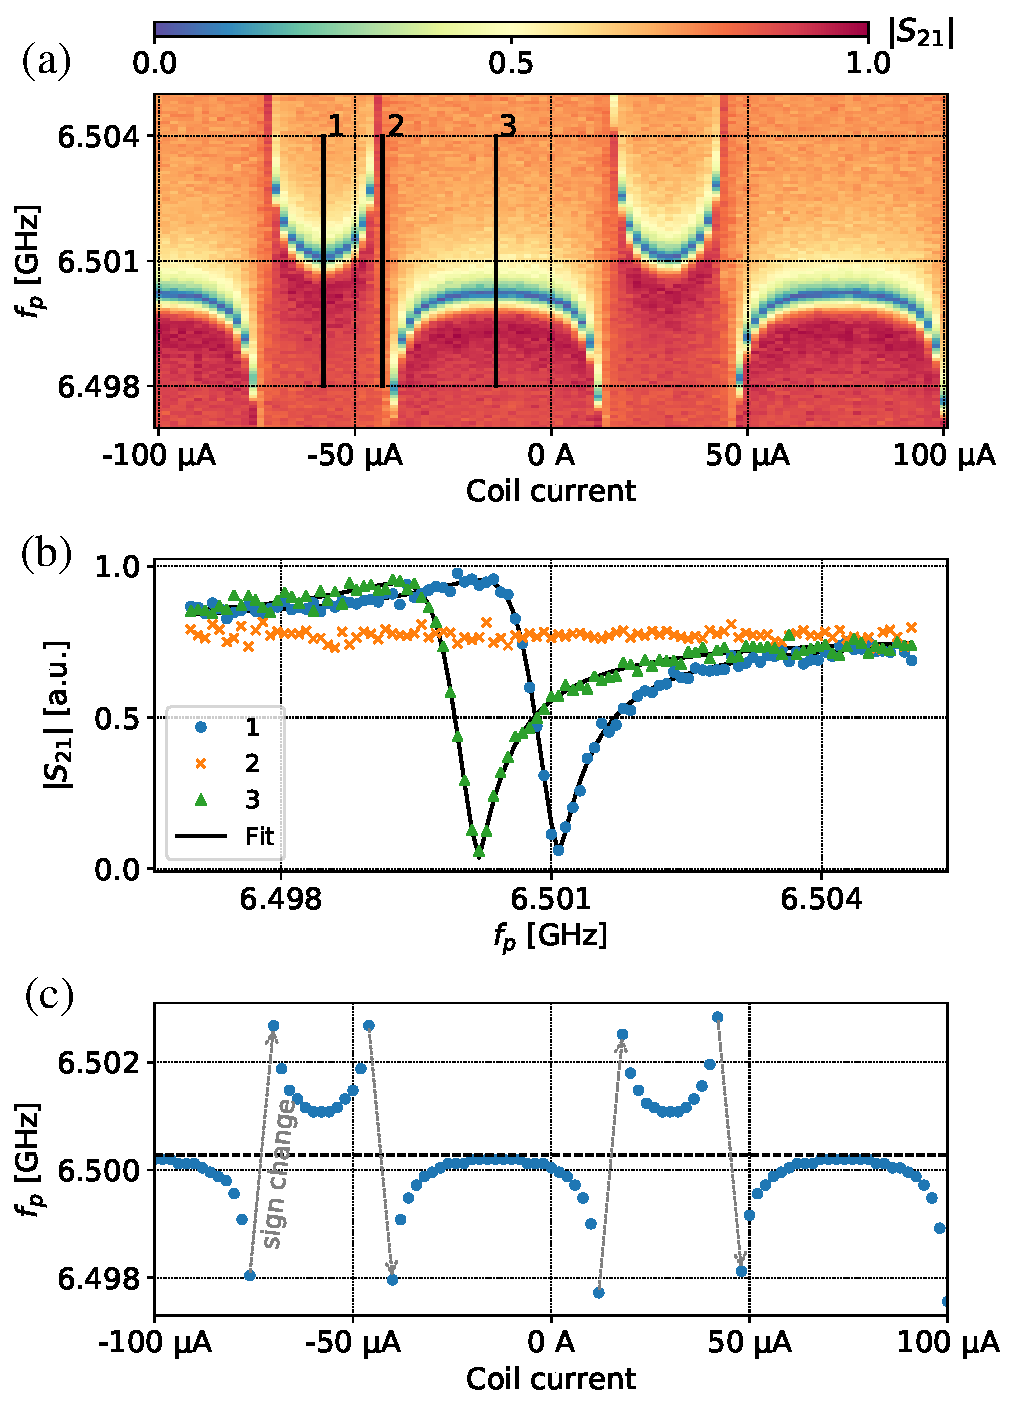
\includegraphics[width=\linewidth]{anti_subplots}
\caption{(a) An experimental spectrum of a resonator strongly coupled to a transmon qubit depending on the coil current $I$. (b) Slices of the transmission from (a) showing two slices with fits (1,3) and a plateau with no dip (2) present. (c) Extracted data (blue dots) and mean frequency value over all points $\langle f_r \rangle_{I}$ (black dashed line). Grey arrows show where $f_r - \langle f_r \rangle_{I}$ changes sign.}
\label{fig:anti_exp}
\end{figure}

To extract the Hamiltonian parameters, we propose to fit the model \eqref{eq:f_r} to the data in \autoref{fig:anti_exp}(a) in the sense of maximum likelihood. However, as one can see, the data are much more complex than the model as it contain an extra dimension\fxwarning{Which dimension? 3-d dimension in heatmap? Why does it makes the task 'much more complex'?}. Even after the dimensionality reduction procedure (described below), the fitting is not a trivial task because the maximum likelihood estimation implicates global optimization.\fxnote{You are trying to say that the difficulty is for the loss function has many local minimums, aren't you?} The situation is even more complicated since the we need to solve an optimization problem with an ill-defined\fxnote{Again, it would be better to say that the loss function is non-linear with many local minima and many parameters rather than ill-defined} loss function (i.e. in the least squares algorithm). This is so, firstly, due to the periodic dependence of the frequencies on current $I$ and the unknown position of the qubit sweet spot $I_{ss}$ and, secondly, due to the strongly non-linear dependence of the model on other parameters. Fortunately, it is possible to get a good initial guess for $\Pi$ and $I_{ss}$ parameters and then brute force search the solution in other variables since we have well defined bounds for each of them. Finally, we can polish the result in all six parameters using a local optimizer.

An outline of the method which uses \autoref{fig:anti_exp}(a) as an example is presented below. As it has already been mentioned, the chosen type of the resonator-qubit arrangement which yields the avoided crossings pattern is not unique: there are two other cases when the qubit spectrum lies entirely below or above the resonator frequency; however, they are treated exactly the same way and are simpler in terms of the loss function behaviour.

\subsection{Extracting $f_r(I)$ from data}\label{sec:extract_fr}

Firstly, we are going to reduce the dimensionality of the data, i.e. extract the resonance frequency for each $I$.

We do this by employing the \textit{circlefit}\cite{probst2015} library which is capable of fitting various types of microwave resonators. For each $I$ we fit the complex transmission $S_{21}(f_p)$ as in \autoref{fig:anti_exp}(b) (solid black lines) and extract the resonance frequency from the model. A possible caveat is that for some $I$ values the resonance dip may disappear (see \autoref{fig:anti_exp}(b)) so the fit will fail. Therefore, such slices are excluded in advance via a threshold condition.

The resulting plot of the extracted resonator frequency versus current $I$ is shown in \autoref{fig:anti_exp}(c) (blue dots). There are some current values located between the branches where the data points are missing, as expected, due to the absence of the resonance. Additionally, we plot here the mean value of the detected frequencies shown as a dashed black line. This parameter is important since it, will firstly, serve as an initial guess for the cavity frequency of the model \eqref{eq:f_r}: $f_c \approx \langle f_r \rangle_{I}$ and, secondly, will be used in the period and phase extraction algorithm which tracks the changes of the sign of the value $\Delta f_r = f_r - \langle f_r \rangle_{I}$ (marked as grey dashed lines in \autoref{fig:anti_exp}(c)). Locating these sign changes allows to find the qubit sweet spot without fittig the full model.

\subsection{Extracting period, phase and sweet spot locations}
\begin{figure}
\centering
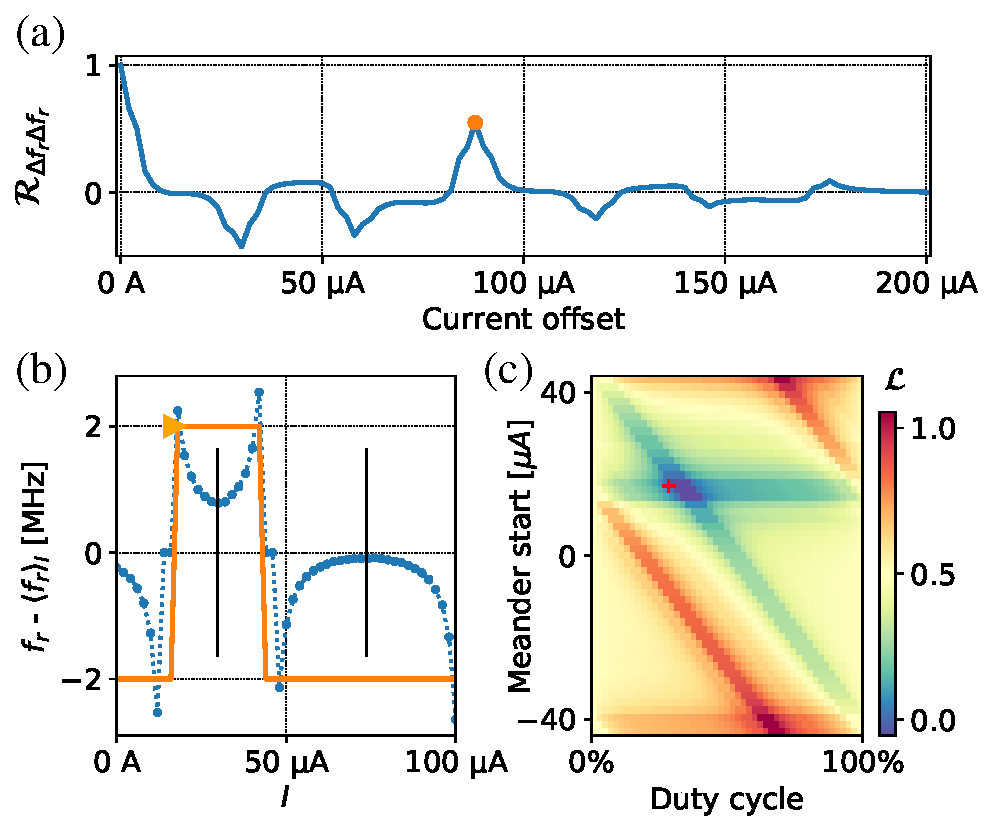
\includegraphics[width=\linewidth]{per+phase}
\caption{Period and phase extraction procedure. (a) Autocorrelation function depending on the current offset $\Delta I$ shows a prominent local maximum at $88\ \mu$A (orange dot). (b) Construction for phase estimation; $\Delta f_r = f_r-\langle f_r \rangle_{I}$ (blue) is fitted with a square wave (orange, start marked with a triangle). Vertical bars mark candidate sweet spots. (c) Loss function (normalized) for the square wave fitting procedure from (b); red cross indicates the parameters of the meander shown there.}
\label{fig:per+phase}
\end{figure}
As we have stated above, one of the serious obstacles for the fitting is the periodicity of the data on one of the fitting parameters. Along with the equally unknown phase of the signal, this leads to the presence of many local minima in the loss function which impede the progress of iterative optimization algorithms. In other words, the unknown parameters $\Pi$ and $I_{ss}$ are preventing us from finding the global minimum. Fortunately, it is possible to determine the period and the sweet spot location (or, the phase of the data) without fitting the full model \eqref{eq:f_r} which alleviates the stated problem. In the absence of noise, this would be a trivial task. However, in the conditions of experiment, the noise to some extent is always present, so below we suggest a solution that is insensitive to local sporadic perturbations of the data.

A powerful tool for finding the period in a given dataset $y$ (especially when it contains just a few periods) is the autocorrelation function $\mathcal{R}_{y y}(l) = \sum_n y_n y_{n-l}$. The location of the largest of its local maxima (except for the $l=0$) equals exactly the sought period. However, this is only true when the mean value of the function is zero; otherwise, $\mathcal{R}_{y y}(l)$ would be linear with a steep slope that may smear out all the extrema. Therefore, instead of directly calculating the autocorrelation of $f_r (I)$ we consider the function $\Delta f_r (I)$ introduced above which has zero mean and the same period. For this function, which looks exactly like one in \autoref{fig:anti_exp}(c) but centered vertically around zero, the autocorrelation function $\mathcal{R}_{\Delta f_r \Delta f_r}(\Delta I)$ depending on the current offset $\Delta I$ is shown in \autoref{fig:per+phase}(a). As one can see, $\Delta I$ spans 200 $\mu$A just as the data itself. This means that to calculate $\mathcal{R}_{\Delta f_r \Delta f_r}(\Delta I)$ the data is being zero-padded at all $\Delta I$ except for $\Delta I = 0$, and this is why we get diminishing correlation peaks at $\Pi$, $2\Pi$, etc. The orange dot in the plot shows the highest local extremum of $\mathcal{R}_{\Delta f_r \Delta f_r}(\Delta I)$ at 88 $\mu$A. It is a very prominent peak and can be easily distinguished among all others. There is as well a small peak at 176 $\mu$A which corresponds to $\Delta I = 2\Pi$. Note that the the autocorrelation function is not ideally smooth and has some abrupt bends on the sides of the peaks. This happens because there were some missing points in the data (corresponding to the plateaus of \autoref{fig:anti_exp}(b)) that were replaced by zeros to ensure the correct mapping between the current indices and current values. This zero padding may be noticed as well in \autoref{fig:per+phase}(b).

Now, having found the period it is possible to precisely determine the phase of the signal. This is done via finding a global maximum of the zero-lag correlation function  $\mathcal{R}_{\Delta f_r S}(0)$ between $\Delta f_r(I)$ and a square wave signal $S(I, \Pi, \phi, D)$ having the same period but unknown phase $\phi$ and duty cycle $D$. The high and low levels of the square must be opposite in value, i.e. 1 and -1, and the absolute value does not matter.  An illustration of a square wave function satisfying the optimal condition is presented in \autoref{fig:per+phase}(b) in orange. The phase $\phi$ (in $\mu$A) denotes the x-coordinate of the first point after the rising edge, and is marked with a triangle. Generally, the idea behind this is to robustly detect sign changes that were shown back in \autoref{fig:anti_exp}(c). We can not rely on a more simple algorithm that walks through the points and marks where the function changes its sign because such algorithm may fail in the presence of noise. Additionally, it will still work correctly even if the mean value $\langle f_r \rangle_{I}$ does not lie exactly between the branches and intersects one of them.

The global optimal $\phi$ and $D$ are found using a brute force algorithm. It calculates the loss function $\mathcal{L} = - \mathcal{R}_{\Delta f_r S}(0)$ on a $50 \times 50$ grid of $(\phi, D)$ and takes the minimal value of all. This method is stable and universal due to the evident boundaries on $\phi \in [-\Pi/2,\Pi/2)$ and $D \in [0, 1]$. The loss function topography for the avoided crossing patterns is nicely structured and for our example is shown in \autoref{fig:per+phase}(c). One peculiarity is that instead of a single minimum it has an area of the same minimal value. Again, this effect comes from the missing zero-padded $f_r$ points at some $I$ values. However, any value from this valley suits well enough for our purposes, and the algorithm finds no difficulty in locating it.

Having found values for $\Pi,\ \phi$ and $D$ we now can calculate the currents of the transmon sweet spots in the case of the avoided crossings pattern and the smooth patterns:
\begin{align}
I_{ss} = 
\begin{cases}
 \phi + \Pi (1+D)/2,\ \text{for the avoided crossings}\\
 \phi + \Pi D/2 ,\ \text{otherwise}
\end{cases}
\end{align}
To distinguish between these two cases when the noise is not too large, one may calculate the maximal absolute differential of the frequency data $\max_{i>0} |f_{r,i} - f_{{r,i}-1}|$ and compare it to the peak-to-peak amplitude $\max_{i,j} | f_{r,i} - f_{r, j}|$. For the avoided crossings these values are close and for the smooth dependencies they are not. However, in the presence of noise this indicator may fail, and one will have to check both current values to be $I_{ss}$ by fitting the full model two times, and then choose among the two possibilities based on the loss value.


\subsection{Full model fitting}

\begin{figure}
\centering
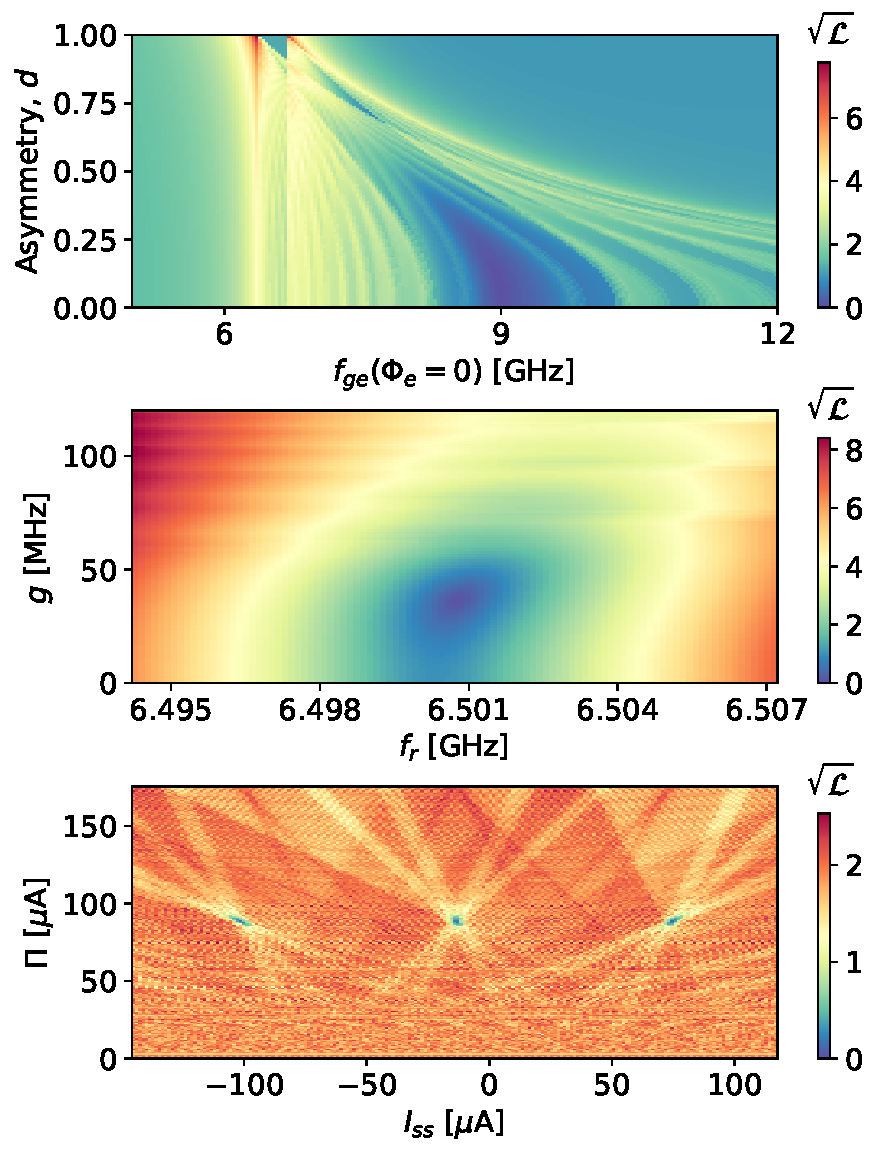
\includegraphics[width=\linewidth]{loss1}
\caption{Slices of the loss function \eqref{eq:loss} for the full model and experimental data from the example made around the optimal point. Root-mean-square per-point loss $\sqrt{\mathcal{L}}$ is in MHz. (a) $f_{ge}^{max}$ and $d$ are varied, other parameters optimal. A large valley is located near 9 GHz, and some smaller locally minimal ones are present all around. (b) $g$ and $f_r$ are varied, others optimal. The loss function for these two parameters is well-conditioned near the optimum. (c) Period $\Pi_{f_r} = \Phi_0/M$ and $\Phi_r/M$ varied, others optimal. This subplot illustrates a complex structure of local minima around the true one which we find analytically.}
\label{fig:loss}
\end{figure}

 
Having performed the aforementioned preliminary steps, it is now possible to fit the full model to the extracted points. To do this, we employ brute force optimization combined with the Nelder-Mead simplex downhill algorithm\cite{nelder1965} to polish the brute force result. For both methods, we use a common loss function defined as follows. For the known probe frequency span of the data $\Delta f_p$ (\autoref{fig:anti_exp}(a), whole y-axis) and the set of $N$ extracted points $\{p_i\} = \{(I_i, f_{r,i})\}$, we calculate the loss function as
\begin{align}
\mathcal{L} &= \frac{1}{N}\sum_{i=0}^N [f_{r,i} - \mathcal{M}(I_i,\ \Pi, \ I_{ss},\ f_c,\ g,\ f_{ge}^{max},\ d)]^2,\label{eq:loss}\\
\mathcal{M} &= \begin{cases}
f_+,\  |f_+ - f_c|< \Delta f_p/2 \\
f_-,\ \text{otherwise}, \label{eq:cond}
\end{cases}
\end{align}
where, as in the previous section, $$f_{\pm}(I_i) = f_{\pm}(I_i,\ \Pi,\ I_{ss},\ \ f_c,\ g,\ f_{ge}^{max},\ d)$$
The condition of Eq. \eqref{eq:cond} means that we choose only the model frequencies that lie within a window $\Delta f_p$ around the model $f_c$ parameter. This ensures, firstly, that in the optimum we will not take any excess points outside the frequency scan, and, secondly, that we have a single model value for each current.

To substantiate the choice of the optimization algorithms, we present in \autoref{fig:loss} three visualizations of the the defined loss function. The plots show how the function behaves if a certain pair of 6 model parameters is varied while others are optimal. From the plots it is obvious that the loss function is ill-defined and has a lot of local minima. Moreover, it may not be smooth everywhere because of the condition \eqref{eq:cond}. The $f^{max}_{ge}$ and $d$ parameters present the most significant difficulty in terms of false minima as can be seen from \autoref{fig:loss}(a). In contrast, $f_c$ presents the least difficulty, as can be seen from \autoref{fig:loss}(b). The last plot \autoref{fig:loss}(c) shows a very complex structure of the loss function and narrow optimal valleys and serves as an illustration of why the period and phase extraction algorithm is important.

\begin{table}
	\centering
	\begin{ruledtabular}
		\begin{tabular}{ccc} 
			Parameter & Value range & Steps \\ 
			\hline
			$f_c$ & $\langle f_r \rangle_{I} \pm 1$ MHz & 3\\ 
			$g$ & 20 - 40 MHz & 5\\
			$f_{ge}^{max}$ &  4 - 12 GHz & 80 \\
			$d$& 0 - 0.9 & 9
		\end{tabular} 
	\end{ruledtabular}
	\caption{Grid specifications for the brute force algorithm for STS detection.}
	\label{tab:grid}
\end{table}

The brute force algorithm acts on the grid specified in \autoref{tab:grid}. The ranges in the grid are based on the usual design parameters of the qubit samples in our database and the number of steps is chosen so that the algorithm reliably finds the optimal valley. After the coarse brute force optimization is done and the optimal valley is located, we apply the Nelder-Mead search on all 6 parameters.


\section{Results}

In this section, we discuss the performance and accuracy of the two algorithms described in the previous section. Firstly, we test the resonator spectrum recognition, and then the qubit spectrum detection algorithm.

The algorithm was implemented in Python using the \textit{brute} and \textit{minimize} routines of the SciPy\cite{scipy} library. We present here three examples of the detection for all possible qubit-resonator dispositions.  The resulting fits are presented in \autoref{fig:anti_fit_cases} along with the original data and the error plots; we will further reference them as (a), (b) and (c). 

The chosen algorithm order works as expected, as one can see from \autoref{tab:sts_results} comparing the brute estimation and  the final result after Nelder-Mead is performed. 	The significant improvement in the loss value of the polished result compared to the brute estimation is due to the more accurate determination of the cavity frequency $f_c$ which leads as well to major shifts in optimal $g$, $f_{ge}^{max}$ and $d$. However, even these optimal qubit parameters and coupling strength may be inaccurate even on GHz scale. For example, in case (b) for $f_{ge}^{max}$ we see a 300 MHz difference between the optimal and the correct value found with TTS. For (a) and (c), the differences in $f_{ge}^{max}$ are much smaller (about 10-70 MHz) but instead we see significant errors in $d$. Inaccuracy in the qubit parameters is caused by low sensitivity of the resonator frequency to the qubit frequency when they are far away and by 

Finally, The match is almost perfect, and the noise in the residuals is random and thus shows no systematic errors. In \autoref{fig:noise_test} we also present the fitting results for different powers of added noise. The signal-to-noise ratio (SNR) is defined for our data in a similar manner as the SNR in the resonator fitting tests\cite{probst2015}; we take distance $2r$ between two maximally remote points of $S_{21}(f_p, I)$ among any pair on the complex plane (i.e., the diameter of the resonance circle) as the signal amplitude, and the noise of the form $\frac{\xi_1+i\xi_2}{\sqrt 2}$, where $\xi_1,\ \xi_2$ distributed normally with zero mean and variance (amplitude) $\sigma$. The SNR then is defined as $r/\sigma$. As one can see from the graph, the algorithm stays robust even at very low SNRs that are even lower than the low limit SNRs for the \textit{circlefit} stability. This is possible because a fallback strategy of taking the smallest amplitude point as the resonance is applied when \textit{circlefit} fails. Ultimately, the key point of this stress test is to show that the algorithm can be applied in real-life scenarios when the data may be of low quality.
\begin{table}[b]
	\centering
	\begin{ruledtabular}
		\begin{tabular}{c|cc|cc|cc} 
			\multirow{2}{*}{Parameter} & 
			\multicolumn{2}{c}{(a)} & 
			\multicolumn{2}{c}{(b)} & \multicolumn{2}{c}{(c)}\\
			& Brute & N-M & Brute & N-M & Brute& N-M\\
			\hline
			$f_c$, GHz &6.5004 & 6.5007 & 6.962 & 6.9628 &  6.47 & 6.465\\ 
			$g$, MHz & 24 & 36.1 & 28 & 43.8 & 36 & 86.5\\
			$f_{ge}^{max}$, GHz & 8 &8.97 &9.2& 9.38& 6.3& 5.89\\
			$d$ &0.5&0.09&0.6&0.61&0.1& 0.325 \\\hline
			Loss, kHz & 251 & 24 &313& 39 &2050& 158
		\end{tabular} 
	\end{ruledtabular}
	\caption{Optimal parameters (rounded) found for the three cases in \autoref{fig:anti_fit_cases} after the brute and Nelder-Mead optimizations. The correct values for $f_q^{max}$ and $d$ (from TTS) are: (a) 9.04 GHz and 0.26; (b) 9.08 GHz and 0.6; (c) 5.9 GHz and 0.42.}
	\label{tab:sts_results}
\end{table}

\begin{figure*}
	\centering
	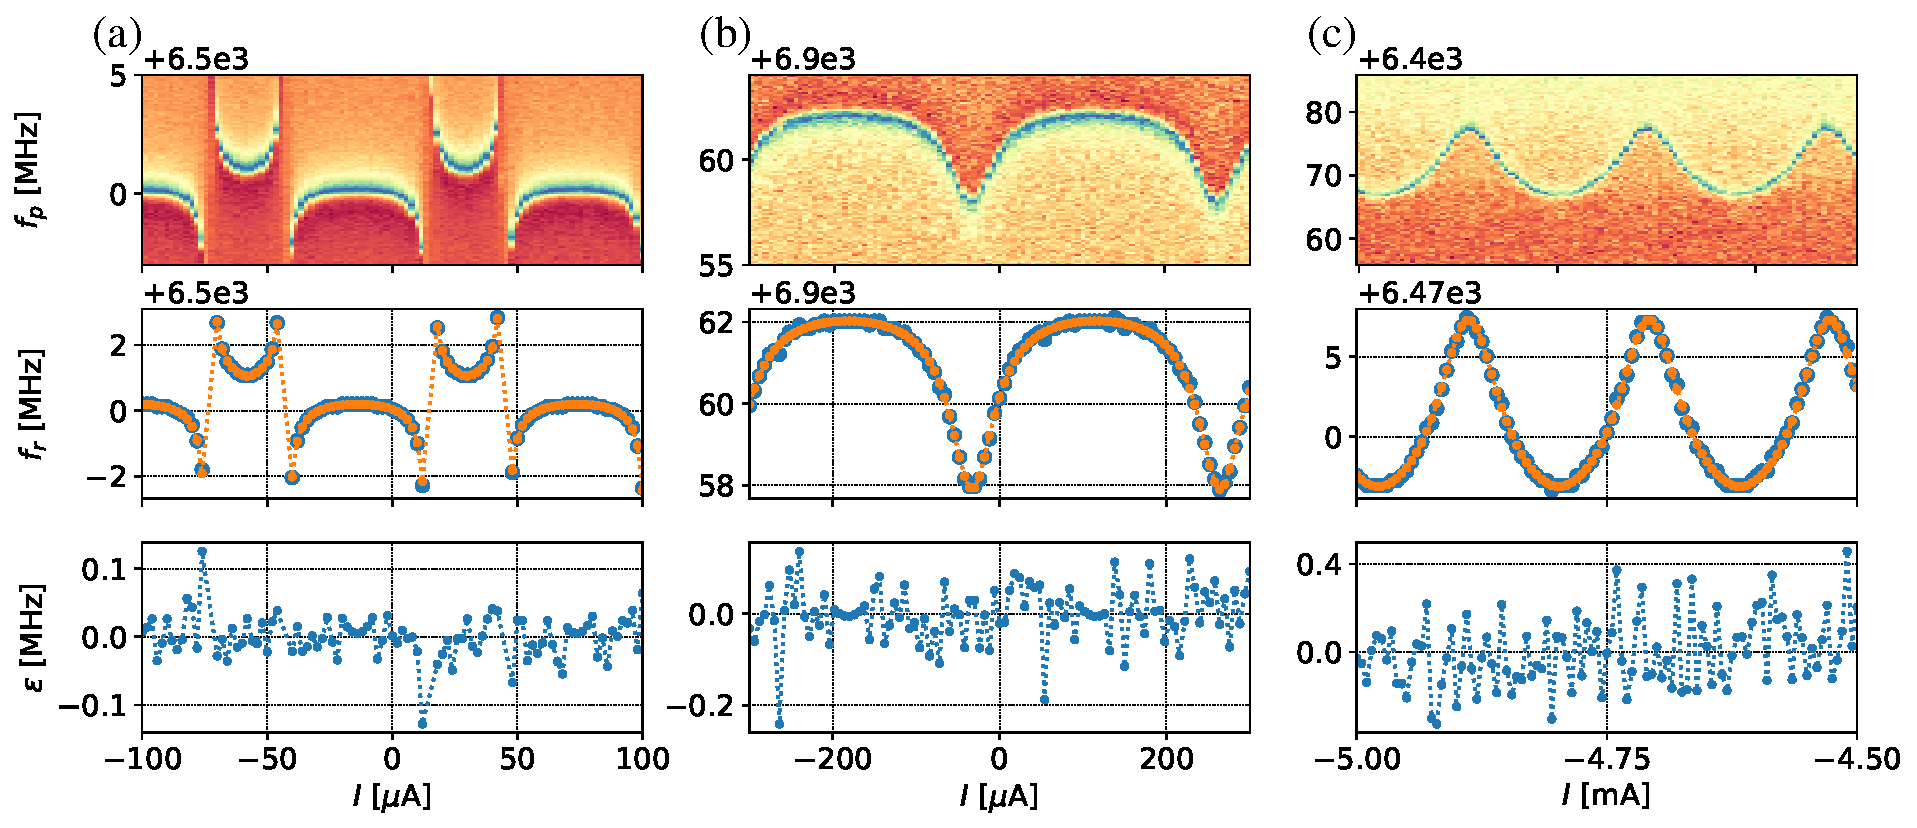
\includegraphics[width=\linewidth]{fit_cases}
	\caption{The results of the algorithm execution on three experimental examples from our database. In the upper row, original images are presented. In the middle row, the data  (blue dots) and the fitted model (orange connected dots) are shown. In the lower row are errors $\varepsilon$. (a) Avoided crossings pattern; per-point RMS error around 30 kHz. (b) The qubit entirely above the resonator; per-point RMS error around 60 kHz. (c) The qubit below the resonator; per-point RMS error around 150 kHz.}
	\label{fig:anti_fit_cases}
\end{figure*}

\begin{figure*}
	\centering
	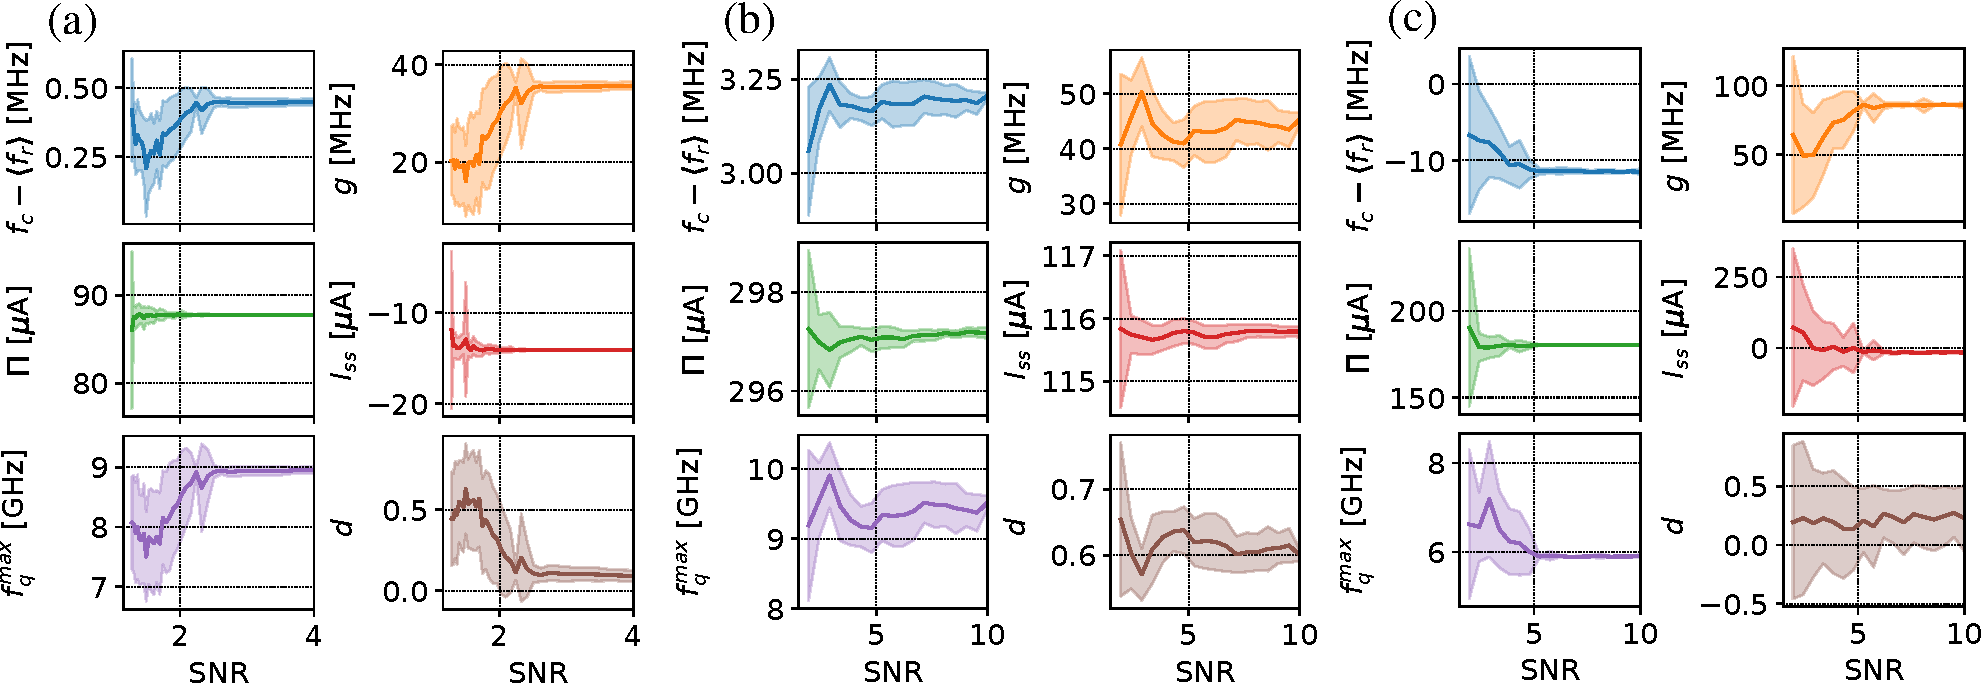
\includegraphics[width=\linewidth]{noise_test}
	\caption{Behaviour of the algorithm on the real data from \autoref{fig:anti_fit_cases} with added gaussian noise of varying power (i.e., with artificially reduced SNR). The clouds show standard deviations of optimal parameters after 50 tries, solid lines show mean values. (a) Detecting avoided crossings; the data used are from \autoref{fig:anti_fit_cases}(a). The algorithm is accurate above SNR=3 but is	 still robust at detecting avoided crossings down to SNR=2 but with reduced accuracy in $f_{ge}^{max}$, $g$ and $d$. (b) Detection for the case of smooth dependence of the resonator frequency on current; the data used are from \autoref{fig:anti_fit_cases}(c). Due to the problems with the resonator fitting, the stability is reached only above SNR=5. Correct qubit parameters $f_{q}^{max}$=5.91 GHz and $d=0.42$ (from TTS); $f_{q}^{max}$ from the fit in the stable region is 5.89 GHz. However, $d$ still can not be determined accurately on the data with noise;it is estimated to be $0.35$ on the original data.}
	\label{fig:noise_test}
\end{figure*}
The fitting example above runs for 3.2 seconds on a 5-year old Intel Core i5-3337U CPU, from which 2.7 seconds are for the brute and 0.4 of a second is for the Nelder-Mead minimization. On a contemporary Intel Core i7-7700 CPU, it takes about one second to run the whole procedure. The time costs mostly come from the square root calculation necessary for Eqs. \eqref{eq:tr_levels} and \eqref{eq:branches2} and because that the brute routine is not parallelized. However, this is still fast, firstly, because recording a resonator spectrum such as one in the example takes around 20 seconds, and, secondly, it is much faster than a human would do. 


\begin{figure}
	\centering
	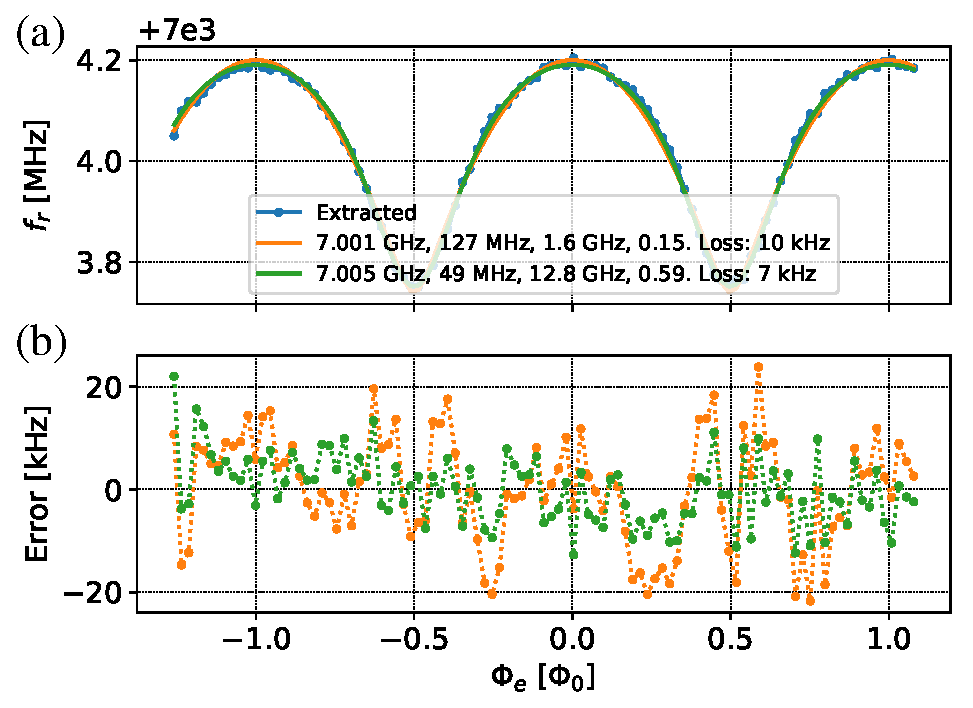
\includegraphics[width=\linewidth]{alternative_fits}
	\caption{(a) Two alternative fits (orange and green lines) for the same data (blue dots). The corresponding parameters $f_c,\ g,\ f_{ge}^{max}, d$ for the two alternative fits are in shown the legend. (b) Residuals for the two fits, in orange (qubit below) and green (qubit above). RMS errors are 14 kHz and 11 kHz, respectively.}
	\label{fig:alternative-fits}
\end{figure}

We have tested the algorithm on more than 100 real spectra that we have in our experimental database, and it finds an optimum for any kind of the dependence of the resonance on the flux caused by various dispositions of the qubit and the resonator, as in \autoref{fig:anti_theor}. Example fitting results for the variants in \autoref{fig:anti_theor}(b,c) are provided in \autoref{fit-other-cases}. There is a caveat, however, in some of such cases. It turns out, that for large qubit-cavity detunings two different sets of parameters minimizing the loss function equally well are possible. An illustration for this statement can be seen in \autoref{fig:alternative-fits}(a),(b). The algorithm was launched using different grid ranges for $f_q^{max}$. In one case (orange) the search was done below, and in the other (green) above the mean resonance frequency $\langle f_c\rangle_{I}$. The resulting fits are equally accurate, and without other information about the system it would not be possible to choose between the two. Therefore, some hints should be passed to the algorithm to avoid ambiguity; for instance, whether to look for the qubit above or below the resonator. Otherwise, it would be necessary to check both possibilities with other methods, i.e. via two-tone spectroscopy.

\section{Discussion}



\appendix



\section{Transmon Hamiltonian}\label{sec:transmon}

The simplest version of this qubit consists of a Josephson junction shunted with a large capacitor. Flux tunability of the frequency is attained by replacing a single Josephson junction with a SQUID as in \autoref{fig:trans}(a) and applying external magnetic flux $\Phi_e$ to its loop. This configuration can be equivalently represented with a shunted junction of tunable energy, \autoref{fig:trans}(b). The Hamiltonian for such equivalent circuit is as follows: 
\begin{equation}
\hat{H}_{tr} = 4E_C \hat n^2 - E_J(\Phi_e) \cos \hat\varphi,
\label{eq:tr_ham}
\end{equation}
where $E_{J1,2}$ are the Josephson energies , $E_C = e^2/2C_{\Sigma}$, $C_{\Sigma} = C_s + C_1 +C_2$, is the charging energy, $\hat n$ and $\hat \varphi$ are the operators for the Cooper pair number and the phase of the qubit island. For the equivalent Josephson energy $E_{J}$ one obtains
\begin{equation}
E_{J}(\Phi_e) = E_{J\Sigma}\cos\left(\pi \Phi_e/\Phi_0\right) \sqrt{1+d^2 \tan^2 \left(\pi \Phi_e/\Phi_0\right)},
\label{eq:EJ_Phie}
\end{equation}  
where $E_{J\Sigma} = E_{J1}+E_{J2}$, $d = \frac{E_{J1}-E_{J2}}{E_{J1}+E_{J2}}$ is the asymmetry of the SQUID. As one can notice, the dependence is periodic in $\Phi_e$.
\begin{figure}
	\centering
	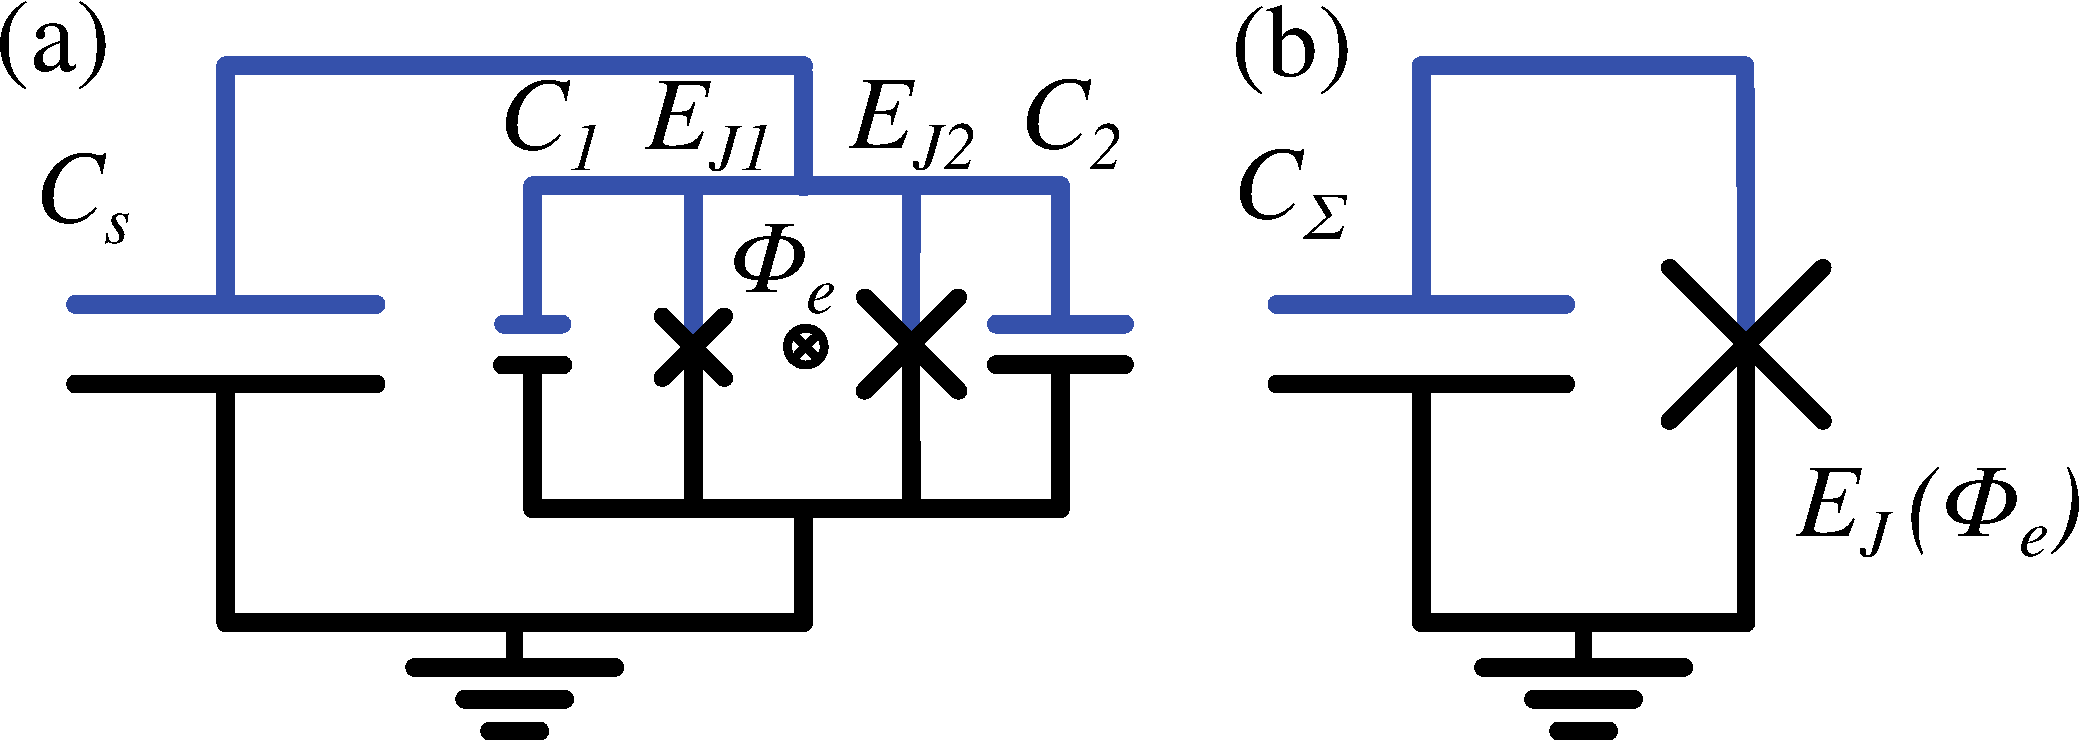
\includegraphics[width=\linewidth]{transmon}
	\caption{(a) A tunable transmon circuit with an asymmetric SQUID, $E_{J1} \neq E_{J2}$. (b) Equivalent transmon with tunable energy $E_{J}(\Phi_e)$ and unified capacitance $C_{\Sigma}$. The qubit island containing its single degree of freedom is in blue.}
	\label{fig:trans}
\end{figure}
\begin{table}
	\centering
	\begin{tabular}{l|c}
		Level & Energy\\
		\hline
		$g\ (E_0)$ & 0\\
		$e\ (E_1)$ & $\sqrt{8E_J E_C} - E_C$\\
		$f\ (E_2)$ & $2\sqrt{8E_J E_C} - 3 E_C$\\
		$d\ (E_3)$ & $3\sqrt{8E_J E_C} - 6 E_C$\\
		$E_4$ & $4\sqrt{8E_J E_C} - 10 E_C$\\
		\hline
	\end{tabular}\quad
	\begin{tabular}{l|c}
		Transition & Frequency\\
		\hline
		$ge$ & $\omega_{ge}$ \\
		$gf/2$ & $\omega_{ge} - 0.5 E_C$\\
		$ef$, $gd/3$& $\omega_{ge}-E_C$\\
		$ed/2$ & $\omega_{ge} - 1.5 E_C$\\
		$fd$, $e E_4/3$ & $\omega_{ge}-2 E_C$\\
		\hline
	\end{tabular}
	\caption{Energies and some transition (single and multi-photon) frequencies for the first 5 levels of the transmon calculated with \eqref{eq:tr_levels}.}
	\label{tab:tr_transitions}
\end{table}
It is also possible to derive analytical expressions for the energy levels and transition frequencies for this type of qubits. The energy of the $m$\textsuperscript{th} level is \cite{koch2007}
\begin{equation}
E_m = m \sqrt{8E_J(\Phi_e) E_C} -\frac{E_C}{12}(6m^2+6m),
\label{eq:tr_levels}
\end{equation}
and some of the transition frequencies are presented in \autoref{tab:tr_transitions}. The qubit frequency  may be approximated as 
\begin{equation}
\begin{aligned}
f_{ge}(\Phi_e) &\approx \sqrt{8 E_J (\Phi_e) E_C} \\
&= f_{ge}^{max} \sqrt{\cos\left(\pi \Phi_e/\Phi_0\right) \sqrt{1+d^2 \tan^2 \left(\pi \Phi_e/\Phi_0\right)}},
\end{aligned}
\end{equation}
where $f_{ge}^{max} = \sqrt{8 E_J(0) E_C}$. This simplifies the expression for the frequency since now it depends on two parameters instead of three.

One final note is that in real-life applications is not possible to know directly the flux $\Phi_e$ that is threaded through the SQUID. The experimenter usually knows only the current $I$ (or voltage) which he applies to some coil that is connected inductively to the SQUID. Then $\Phi_e = M I + \Phi_r$, where $M$ stands for the mutual inductance of the coil and the SQUID, and $\Phi_r$ is some residual flux inherent to the sample.

\section{Circuit QED}\label{sec:cqed}


\begin{figure*}
	\centering
	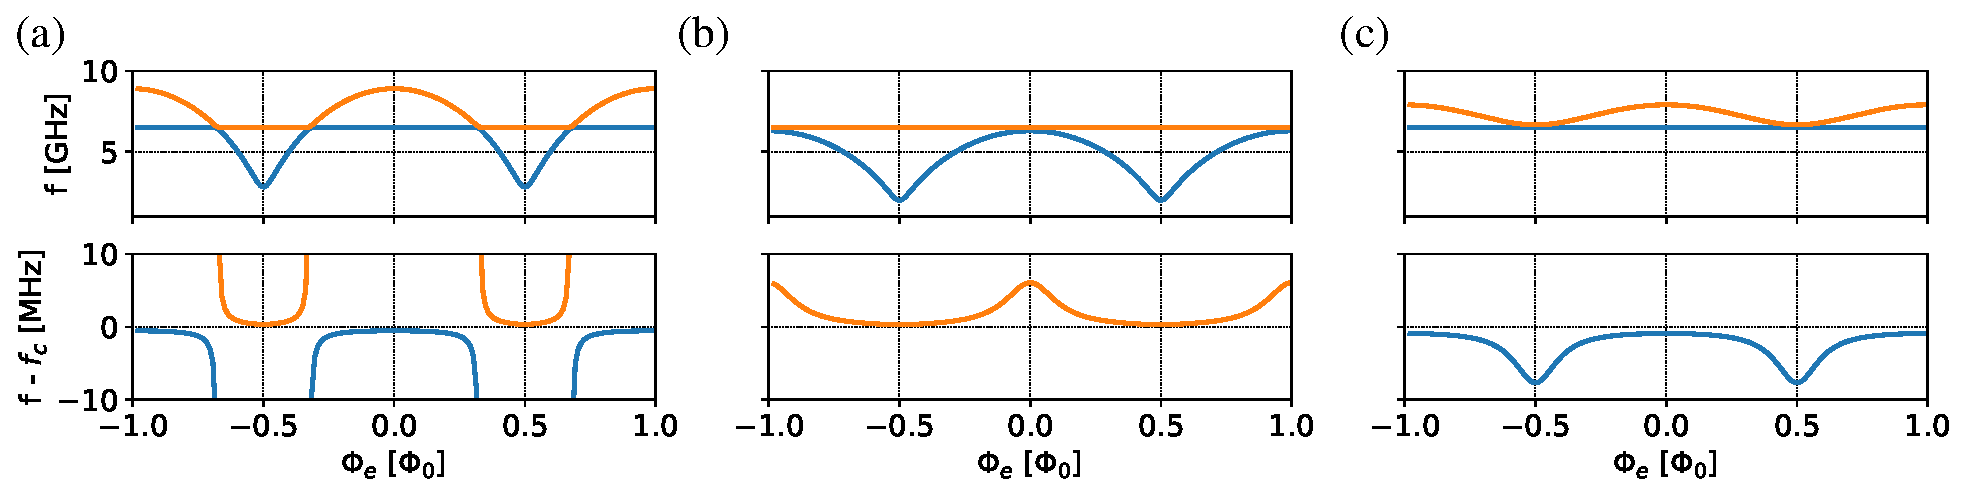
\includegraphics[width=\textwidth]{anti_theor}
	\caption{Frequency spectrum of the transmon-resonator system. Parameters used: $f_{ge}(0) \approx \sqrt{8E_C E_J(0)}/2\pi = 8.5$ GHz, $d=0.3$, $f_r=6.4$ GHz, $g = 30$ MHz. For each subplot two transition branches  $f_{\pm} = (E_{\pm,0} - E_{g,0})/2\pi$ are shown (orange and blue, respectively) both forming the resonator and qubit lines. As one can notice, there are three qualitatively different cases of the resonator-qubit disposition. Lower row shows a zoomed area around $f_c$ that looks differently in each case.}
	\label{fig:anti_theor}
\end{figure*}

The readout of the superconducting qubits is now predominantly done using an ancilla system which is usually implemented as a superconducting microwave resonator which acts as an electromagnetic cavity in the standard cavity QED. Truncating the qubit to two levels, one may obtain the following Hamiltonian for the compound cavity-qubit system (in RWA):
\begin{equation}
\hat H/h = \frac{f_q}{2} \hat \sigma_z + f_c \hat a^\dagger \hat a + g(\hat \sigma^- \hat a^\dagger + \hat \sigma^+ \hat a),
\end{equation}
where $f_q$ is the qubit frequency, $f_c$ is the cavity frequency and $g$ is the coupling strength. As long as the RWA is done, this Hamiltonian may be diagonalized analytically\cite{blais2004}:
\begin{align}
E_{g, 0}/h &= \frac{f_c - f_q}{2},\label{eq:branches1}
\\
E_{\pm, n}/h &= (n+1)f_c \pm \frac{1}{2}\sqrt{4g^2(n+1)+(f_q-f_c)^2}.
\label{eq:branches2}
\end{align}

This is very convenient for our purposes. By substituting the dependence of the qubit frequency $f_q \equiv f_{ge}(\Phi_e)$ into these equations, we can get straightforwardly the full system spectrum in dependence on the magnetic flux. In \autoref{fig:anti_theor} we have used the equations \eqref{eq:tr_levels}, \eqref{eq:branches1} and \eqref{eq:branches2} to model a tunable transmon interacting with a cavity for various $\Phi_e$ and various $f_{ge}^{max},\ d$. In the lower row of the figure, one can see that it is possible to extract the dependence of the \textit{cavity} frequency $f_c$ on $\Phi_e$; for example, the well-known avoided crossing pattern can be directly observed in \autoref{fig:anti_theor}(a), and the other two possible behaviours for the qubit entirely above or below the resonator in \autoref{fig:anti_theor}(b),(c). To shorten the notation, in the following we will define the corresponding branch frequencies of \eqref{eq:branches2} as $f_{\pm} = ( E_{\pm,0}-E_{g,0})/2\pi$.

In \autoref{fig:anti_theor}(a) it is also possible to see the entire spectrum of a transmon $ge$ transition predicted by equations \eqref{eq:EJ_Phie}, \eqref{eq:tr_levels}. It has a cosine-like periodic shape with a period of one flux quantum $\Phi_0$. Consequently, it has two extrema, the upper and the lower which are called ``sweet spots'' due to the first-order insensitivity to $\Phi_e$, and thus to possible flux noise. In the following, by saying sweet spot we will assume the upper one whose frequency is $f_{ge}(\Phi_e = 0) \equiv f^{max}_{ge}$ .

We will use the model \eqref{eq:branches1}, \eqref{eq:branches2} to fit the resonator frequency that we can find in an experiment. The only conceptual problem for the fitting that is left now is that the function we want to use as a model is not single-valued. Indeed, in \autoref{fig:anti_theor}(a, top) for each value of magnetic flux we always find two frequency points corresponding to the qubit and to the resonator, respectively. However, in practice only a narrow scan around the resonator frequency such as in \autoref{fig:anti_theor}(a, bottom) is required, and thus no ambiguity occurs. 

\bibliography{papers_bibliography}% Produces the bibliography via BibTeX.
\listoffixmes
\end{document}
%
% ****** End of file aipsamp.tex ******